\documentclass[11pt,spanish]{article} % Idioma
\usepackage{babel}
\usepackage[T1]{fontenc}
\usepackage{textcomp, verbatim} % \begin{comment}
\usepackage[utf8]{inputenc} % Permite acentos

\usepackage{wrapfig} % Imagenes %\graphicspath{ {./imagenes/} }
\usepackage[left=2.75cm,top=2.5cm,right=2cm,bottom=2.5cm]{geometry} % Márgenes
\usepackage{amssymb, amsmath, amscd, amsfonts, amsthm, mathrsfs } % Símbolos matemáticos
\usepackage{cancel} % Cancelar expresiones
\usepackage{multirow, multicol, tabularx, booktabs, longtable} % Tablas
\usepackage{fancyhdr, fncychap} % Encabezados
\usepackage{algpseudocode, algorithmicx, algorithm} % Pseudo-código	
\usepackage{bbding} % Símbolos
\usepackage{enumitem} % Enumerados a), b), c)... usando \begin{enumerate}[label=\alph*)]
\usepackage{graphicx, xcolor, color, pstricks} % Gráficos --TikZ-- 
% http://www.texample.net/tikz/examples/
\usepackage[hidelinks]{hyperref}  % Enlaces
\usepackage{verbatim} % Comentarios largos \begin{comment}
\usepackage{rotating} % \begin{rotate}{30}
\usepackage[all]{xy} % Diagramas
\usepackage{listings} % Escribir código 
\usepackage{xparse} % Entornos


% Comandos
\newcommand{\docdate}{}
\newcommand{\subject}{}
\newcommand{\docauthor}{Rubén Morales Pérez}
\newcommand{\docemail}{srmorales@correo.ugr.es}

\newcommand{\N}{\mathbb{N}}
\newcommand{\Q}{\mathbb{Q}}
\newcommand{\C}{\mathbb{C}}
\newcommand{\R}{\mathbb{R}}
\newcommand{\Z}{\mathbb{Z}}


\linespread{1.1}                  % Espacio entre líneas.
\setlength\parindent{0pt}         % Indentación para párrafo.

\title{Prácticas Fundamentos de Redes: \\ Chromecast}
\author{Francisco Javier Morales Piqueras \\
		María Florencio \\
		Rubén Morales Pérez}
\date{\today}

% % % % % % % % % % % % % % % % % % % % % % % % % % % % % % % % %
%					 Inicio del documento
% % % % % % % % % % % % % % % % % % % % % % % % % % % % % % % % %
\begin{document}

\maketitle
\tableofcontents % Generando el indice
\newpage
\setlength\parindent{0pt} % Quitamos la sangría


\section{Introducción}
\section{Introducción}
Google Chromecast es un dispositivo de reproducción multimedia fabricado por Google y comercializado a partir de Julio de 2013. Reproduce contenido multimedia conectado a una televisión o monitor vía HDMI haciendo streaming mediante Wi-Fi. Un nuevo modelo Chromecast Ultra que soporta 4k fue anunciado durante el evento \#MadeByGoogle.

\

Para hacer streaming utiliza el software Google Cast, un protocolo propietario de Google que permite controlar la reproducción de contenido multimedia desde un dispositivo local en otro dispositivo compatible con esta tecnología. Google Cast dispone de librerías para las últimas versiones de Android y iOS, así como para Chrome OS y aplicaciones de Google Chrome.

\begin{figure*}[h]
	\centering
	\begin{minipage}[b]{.35\textwidth}
		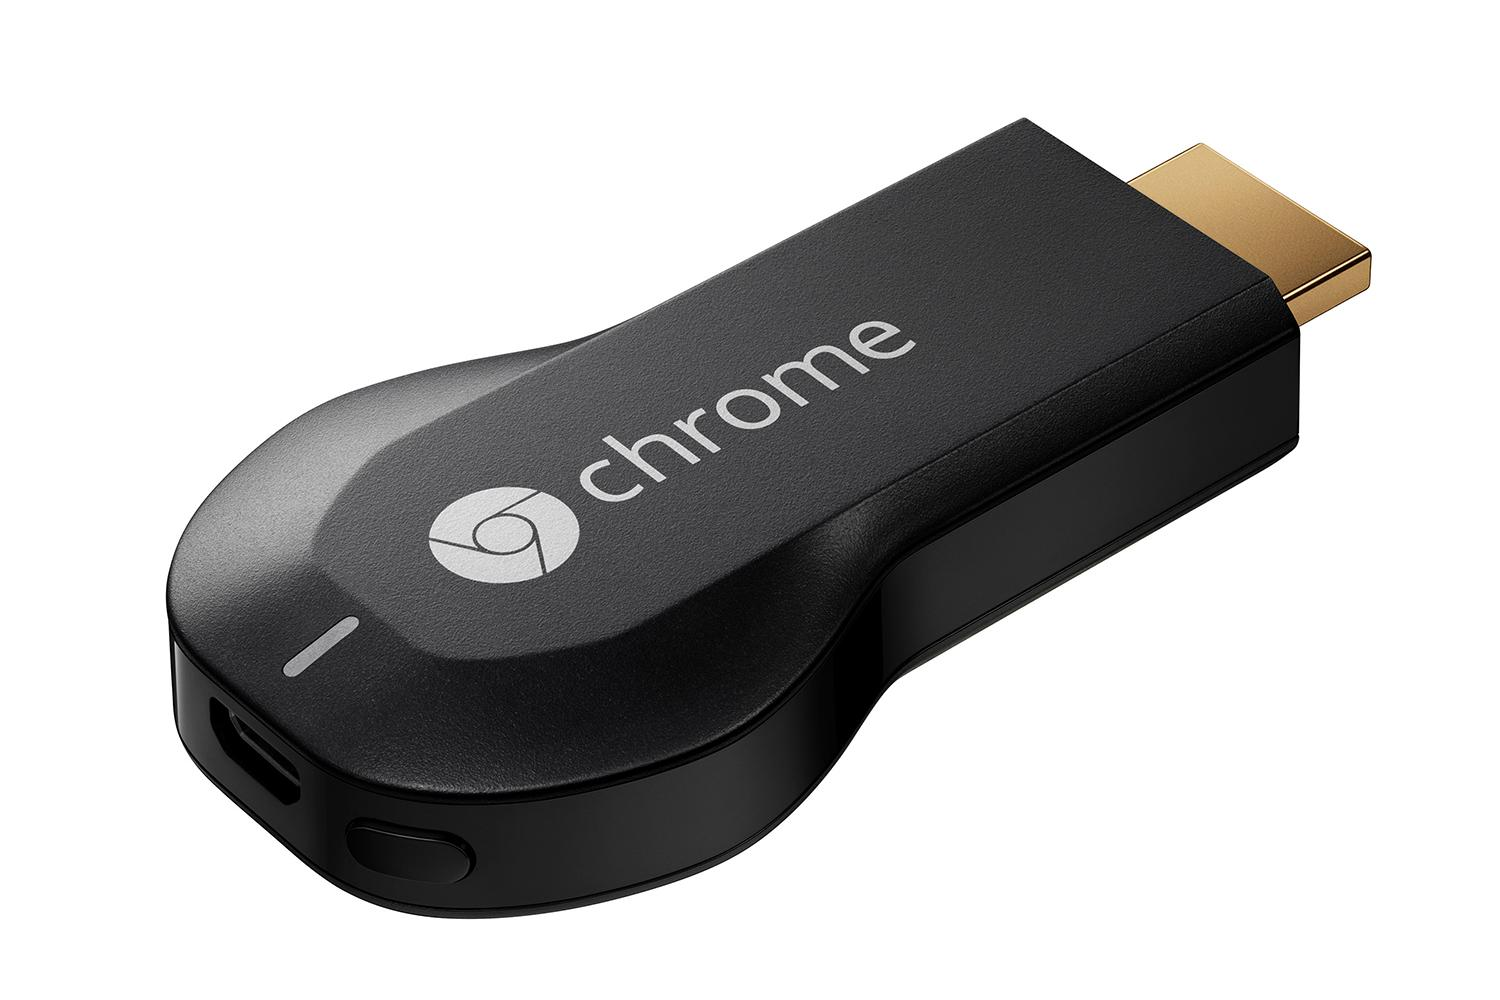
\includegraphics[scale=0.11]{./Imagenes/chromecast1gen.jpg}
		\caption{Primera generación}\label{fig:1gen}
	\end{minipage}\qquad
	\hspace{1cm}
	\begin{minipage}[b]{.35\textwidth}
		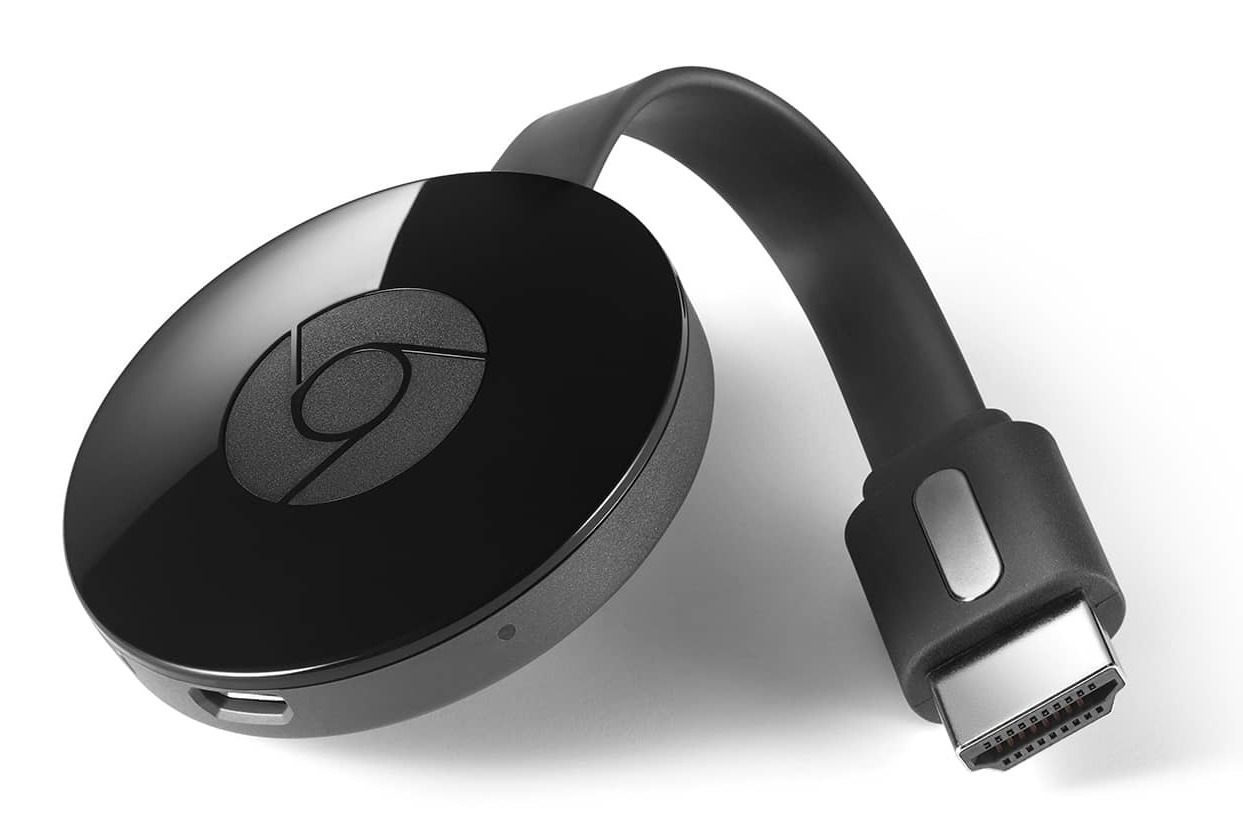
\includegraphics[scale=0.15]{./Imagenes/Chromecast.jpg}
		\caption{Segunda generación}\label{fig:2gen}
	\end{minipage}
\end{figure*}

Chromecast permite reproducir contenido almacenado en un dispositivo conectado a la red local o en un sevidor externo. El control de la reproducción se realiza en ambos casos desde uno o varios dispositivos locales compatibles con la tecnología Google Cast.

\

Cuando no hay contenido en streaming reproduce un contenido personalizable de fondo, puede incluir fotos personales,
de satélite, noticias, etc. Por defecto muestra imágenes aleatorias seleccionadas por Google.

\

Su principal competidor es el servicio AirPlay desarrollado por Apple, que permite streaming inalámbrico entre dispositivos iPhone, iPad o Mac para audio, vídeo, fotos, etc.

\vspace{1cm}
\begin{figure}[h]
	\centering
	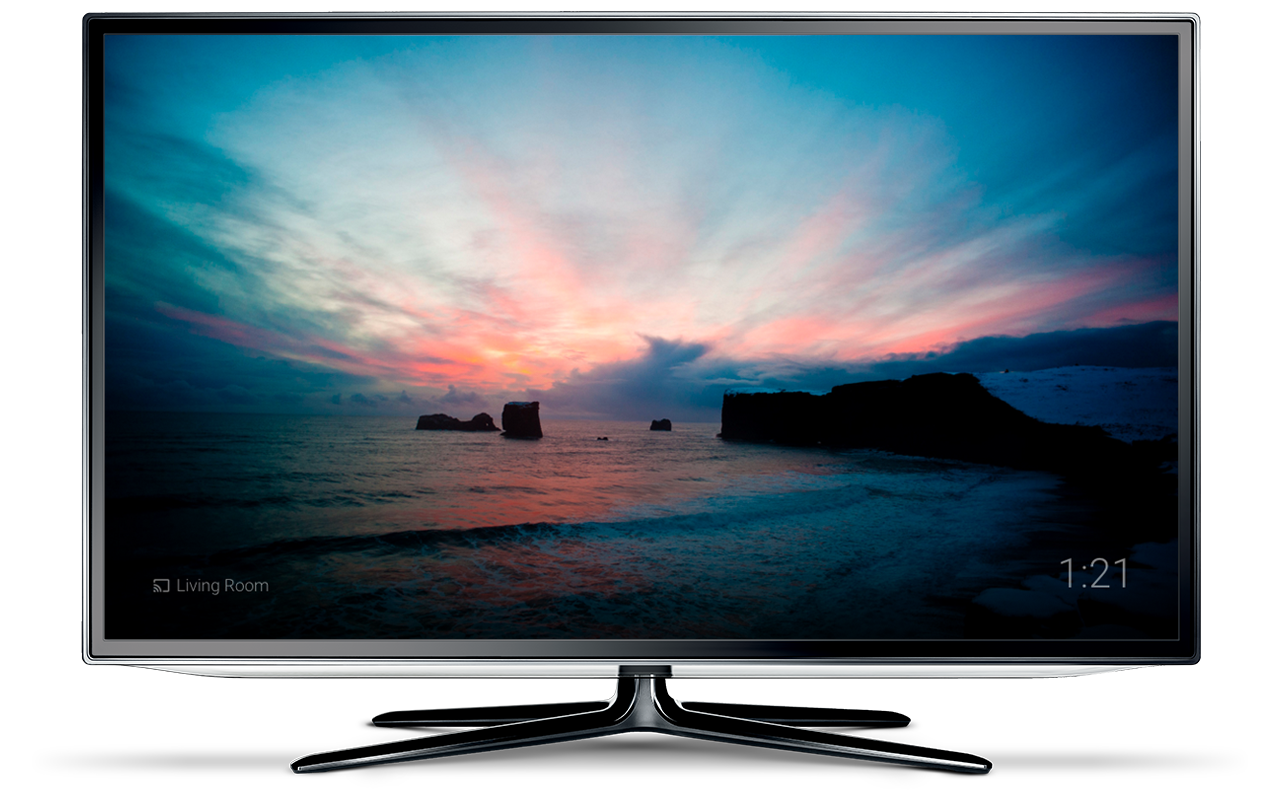
\includegraphics[width=0.6\textwidth]{./Imagenes/fondo.png}
	\label{fig:fondo}
\end{figure}

\newpage


\subsection{Generaciones}

El chromecast de primera generación incluye un decodificador de VP8 y H.264 para formatos de compresión de vídeo, 512 MB de Micron DDR3L RAM y 2 GB de memoria flash.
El de segunda generación tiene un cable flexible y magnético, usa procesador dual ARM Cortex-A7 de frecuencia 1.2 GHz y tiene tres antenas adaptativas para mejroar la conexión con el router.
El dispositivo tiene 512 MB de Samsung DDR3L RAM y 256 MB de memoria flash.

%%%%%%%%%%%%%%%%%%%%%%%%%%%%%%%%%%%%%%%%%%%%%%%%%%%%%%%%%%%%%%%%%%%%%%%%%%%%%%%%%%

% % % % % % % % % % % % % % % % % % % % % % % % % % % % % % % % %
%					 Bibliografía
% % % % % % % % % % % % % % % % % % % % % % % % % % % % % % % % %

\end{document}
